\section{Simulazione e esperienza in laboratorio}
\label{sec:simLab}

	In questa sezione si confrontano i dati ottenuti con le simulazioni sul modello del motore e quelli raccolti nell'esperienza di laboratorio con quanto previsto dalla teoria. In particolare si vogliono testare le differenze tra l'uso di un controllore PID con desaturatore, controllo in feed-forward e controllo integrale.
	
	\subsection{Simulazione controllore PID con desaturatore}
	\label{subsec:PIDdesaSim}
	
		Si verificano le prestazioni di un controllo PID con desaturazione in simulazione, utilizzando il modello del motore ricavato nella sezione \ref{subsec:ModellizzazioneMotoriduttore}; in particolare si utilizzano il codice \textit{MATLAB} e i modelli \textit{SIMULINK} riportati rispettivamente nelle appendici \ref{subapp:controllorePID} e \ref{subapp:modelloPID}. 
		\newline Le specifiche da rispettare sono:
		
		\begin{align*}
			t_s &\le 0.30 \singleSpacing [s] \trippleSpacing \textnormal{rispetto a $\pm 1 [gradi]$ del valore a regime} \\
			S &\le 5 \% \\
			r &= 10,50,120 \singleSpacing [gradi] \\
			d &= \pm 0.5 \singleSpacing [Volt] \\
		\end{align*}
		
		\noindent dove $t_s$ è il tempo di assestamento, $S$ è la sovraelongazione in termini assoluti rispetto al valore di
		riferimento e $r$ è l'ampiezza del gradino di ingresso. Si utilizza allora la progettazione in frequenza, come nella sezione \ref{sub:ProgettazionePID} per il calcolo dei parametri PID e \ref{subsec:Desaturatore} per il calcolo del parametro di desaturazione. Ovviamente tale metodologia di progettazione prevede diversi gradi di libertà (la scelta di $\alpha \in [\frac{1}{3},\frac{1}{10}]
		$ e $b \in [4, \infty)$) e introduce delle approssimazioni che possono rendere necessaria una taratura manuale dei parametri. Le simulazioni sono state suddivise per $d=0.5$ e $d=-0.5$, nell'appendice \ref{subapp:PIDsimulazione} si possono osservare tutti i grafici e le tabelle delle simulazioni. Nel primo caso l'uscita del sistema risulta più veloce ma con una sovraelongazione piuttosto marcata, mentre nel secondo è più lenta ma con meno sovraelongazione. Questo si traduce nel fatto che le specifiche non sono rispettate per alcuni segnali di ingresso e si rende necessaria una ritaratura manuale dei parametri. Questa ritaratura però non è del tutto banale, in quanto bisogna diminuire la velocità del sistema per il primo caso e aumentarla nel secondo, si è cercato allora un compromesso. Si è data per prima cosa priorità al tempo di salita per $d=-0.5$ e $r=10$ che superava addirittura il secondo; si è aumentato allora il guadagno integrale per rendere il sistema più veloce. Questo ha però aumentato la sovraelongazione per $d=0.5$ di parecchio, ma per abbassarla si è aumentato anche il guadagno proporzionale, che prima era inferiore all'unità. Alla fine si è dovuto aumentare anche il guadagno proporzionale visto che risultava troppo basso rispetto gli altri due e la sua azione era quasi ininfluente. In conclusione la ritaratura ha portato dei risultati soddisfacenti, riportati nelle figure \ref{fig:PIDd_0_5} e \ref{fig:PIDd__0_5}. Nei grafici si può apprezzare come gli ingressi di controllo saturino quasi subito e sono parecchio instabili, probabilmente dovuto al fatto che i  guadagni integrali sono molto elevati, ma la sovraelongazione rimane comunque bassa grazie all'intervento del desaturatore.
		
		\begin{figure}[H]
			\centering
			\includestandalone[width=1\textwidth]{./simulazioni/4_d_0_5_tuned} 
			\caption{Ingressi di controllo e uscite del motore con controllore PID con desaturatore e rumore additivo $d=0.5$ dopo la taratura manuale.}
			\label{fig:PIDd_0_5}
		\end{figure}
		
		\begin{figure}[H]
			\centering
			\includestandalone[width=1\textwidth]{./simulazioni/4_d__0_5_tuned} 
			\caption{Ingressi di controllo e uscite del motore con controllore PID con desaturatore e rumore additivo $d=-0.5$ dopo la taratura manuale.}
			\label{fig:PIDd__0_5}		
		\end{figure}		
		
		
		
	
	
	
	
	
		
	\subsection{Simulazione controllo in feedforward}	
	\label{subsec:feedforwardSim}
	
		In questo caso si vogliono verificare le prestazioni di un controllo in feedforward per rispettare le seguenti specifiche:

		\begin{align*}
			t_s &\le 0.0.15 \singleSpacing [s] \trippleSpacing \textnormal{rispetto a $\pm 5 \%$ del valore a regime} \\
			S &\le 10  \% \\
			r &= 10,50,120 \singleSpacing [gradi] \\
		\end{align*}	
		
		\noindent Per la sua progettazione, mentre per il guadagno di feedforward si deve applicare semplicemente una formula, per il piazzamento dei poli in catena chiusa si ha più libertà. In questo laboratorio si usa l'\textit{approssimazione ai poli dominanti}, ovvero si approssima il sistema in catena chiusa con uno del secondo ordine. Le matrici del sistema in forma di stato con stato $x=\begin{bmatrix}\theta_l(t) & \dot{\theta}_l(t)\end{bmatrix}^T$ sono:
		
		\begin{align*}
			A\approx
			\begin{bmatrix}
				0 & 1     \\
				0 & -40.3 \\
			\end{bmatrix}
			\trippleSpacing
			B\approx
			\begin{bmatrix}
				0     \\
				375.3 \\
			\end{bmatrix}
			\trippleSpacing
			C\approx 1.6
			\trippleSpacing
			D=0
		\end{align*}
		
		\noindent Inoltre il sistema è controllabile visto che $\det[B|AB]\ne 0$ e allora è possibile trovare una matrice di retroazione $K$. Si deve allora semplicemente trovare $K=\begin{bmatrix}K_1 & K_2 \end{bmatrix}$ che soddisfi la seguente equazione:
		
		\begin{equation}
			\det[sI-(A-BK)] = s^2 + 2\xi\omega_ns+\omega_n^2
			\label{eq:poliDominanti}
		\end{equation} 
		
		\noindent dove i due poli dominanti della parte destra dell'equazione \ref{eq:poliDominanti} sono
		
		\begin{equation*}
			p_{1,2}=-\sigma \pm \jmath\omega_d=-\xi\omega_n\pm\jmath\sqrt{1-\xi^2\omega_n}
		\end{equation*}
		
		\noindent con $\sigma\approx\frac{3}{t_s}$ e $\xi=0.6$ dalla solita tabella di figura \ref{fig:mSxiS}. Quindi i due poli risultano
		
		\begin{align*}
			p_1 &\approx -20 + \jmath 27 \\
			p_2 &\approx -20 - \jmath 27 
		\end{align*}
		
		\noindent e dunque la matrice di retroazione $K$ risulta $K\approx\begin{bmatrix}2.9608 & -0.0008\end{bmatrix}$. Si passa allora alla simulazione, come prima il codice \textit{MATLAB} è presente nell'appendice \ref{subapp:controlloreFF} mentre lo schema \textit{SIMULINK} in \ref{subapp:modelloFF}. Ovviamente quando è presente un rumore additivo $d=\pm 0.2$ il sistema inseguirà il gradino ma avrà un errore a regime non nullo; per eliminarlo bisogna ritarare il termine di feedforward per ogni tipo di ingresso. Una volta fatto questo comunque il sistema risultante rispetta le specifiche proprio al limite. Le uscite risultanti, suddivise per $d=0.2$ e $d=-0.2$ sono riportate in figura \ref{fig:FFd}.
		
		\begin{figure}[H]
			\centering
			\includestandalone[width=1\textwidth]{./simulazioni/5_d_only_out} 
			\caption{Uscite del motore con controllore feedforward e rumore additivo $d=\pm 0.2$ dopo la taratura.}
			\label{fig:FFd}		
		\end{figure}	
		
		% font e linea grafici MATLAB
		\pgfplotsset{every axis/.append style={
			font=\large,
			line width=1pt,
			tick style={line width=0.8pt}}}
					
		\begin{wrapfloat}{figure}{R}{0pt}
			\centering
			\begin{tikzpicture}[scale=0.99]
				\begin{axis}[
				grid=major,
		  		xmin=950, xmax=1300, 
		  		ymin=0, ymax=60,     
		  		xlabel={$t \singleSpacing [s]$},			  		
		  		ylabel={$y \singleSpacing [gradi]$},            
			  	title={Uscite del motore con incertezza nel parametro $a$}, 
			  	xtick={1000,1100,...,1300},
		 		xticklabels={$1$, $1.1$, $1.2$, $1.3$},
		 		ytick={0,10,...,60},
		  		yticklabels={$0$, $10$, $20$, $30$, $40$, $50$, $60$},
		  		y label style={at={(axis description cs:0.1,.5)},anchor=south},
		  		legend style={at={(0.97, 0.7)}, anchor=north east},        
		  		legend cell align=left,     
		  		legend entries={$a=1.1a_{nom}$, $a=1.2a_{nom}$},
				]
					\addplot[red] table {./simulazioni/5/a/out_r_50_a_1_1_a.dat};
					\addplot[green] table {./simulazioni/5/a/out_r_50_a_1_2_a.dat};					
				\end{axis}
			\end{tikzpicture}	
			\caption{Uscite del motore con controllore feedforward e incertezza nel parametro $a$.}	
			\label{fig:FFa}			
		\end{wrapfloat}		
		
		\noindent Se invece si elimina il rumore additivo ma si aggiunge dell'incertezza nella matrice $A$, nel nostro caso $a=1.1a_{nom}$ oppure $a=1.2a_{nom}$, dove $a$ è lo scalare in posizione $(2,2)$ della matrice $A$, il sistema non ha bisogno di ritarature manuali. Infatti rispetta le specifiche ancora meglio che avendo la conoscenza perfetta del parametro $a$; questo può all'inizio sembrare contro intuitivo, ma è spiegabile dal fatto che il posizionamento dei poli in catena chiusa con l'approssimazione ai poli dominanti, introduce appunto approssimazioni, sopratutto se i poli non considerati sono abbastanza vicini a quelli considerati. Per scrupolo si è comunque provato ad aggiungere ulteriore incertezza e, dopo una certa soglia, le prestazioni si abbassano di molto. 
		
		
		
		\leavevmode\newline\newline\newline\newline\newline\newline
	\subsection{Simulazione controllo integrale}
	\label{subsec:ItegraleSim}	
		
		Per ultimo si vuole progettare un controllo integrale per rispettare le stesse specifiche del controllo in feedforward. Con questa tecnica il sistema ha tre stati, come descritto nella sessione \ref{subsec:ControlloIntegrale}, e bisogna decidere allora il posizionamento di tre poli invece di due. Anche in questo caso si considera un sistema del secondo ordine per individuare una regione indicativa per il posizionamento dei poli. Nello specifico si sono provate quattro configurazioni diverse, descritte nella figura \ref{fig:quattroPoli} scegliendo quella migliore per un ingresso $r=50$ e senza disturbo $d$. la figura \ref{fig:quattroPoli} mostra inoltre l'area dove è possibile collocare i poli per soddisfare le specifiche utilizzando l'approssimazione per un sistema del secondo ordine e quindi i valori di $\sigma$ e $\omega_d$ calcolati precedentemente. La configurazione (A) prevede di spostare i tre poli al limite della regione delle specifiche ma sufficientemente distanti tra loro, la (B) invece li posiziona sempre al limite ma tutti nello stesso punto, la (C) invece li posiziona molto all'interno della regione e distanziati tra loro, per ultimo la (D) li posiziona ancora più distanti e un polo è molto negativo.
		
		\begin{figure}[H]
			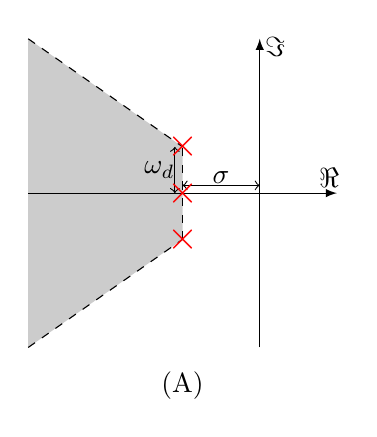
\begin{tikzpicture}[scale=0.98]
				%\draw[help lines,step=1] (0,0) grid (4,4);
				\draw [-latex] (0,2) -- (4,2);
				\draw [-latex] (3,0) -- (3,4);
				\draw [dashed] (0,0) -- (2,1.4);
				\draw [dashed] (0,4) -- (2,2.6);
				\draw [dashed] (2,1.4) -- (2,2.6);
				\draw [<->] (2,2.1) -- (3,2.1);
				\draw [<->] (1.9,2) -- (1.9, 2.6);
				\fill [fill opacity=0.2] (0,0) -- (2,1.4) -- (2,2.6) -- (0,4);
					
				\node [align=center] at (3.9, 2.2) {$\Re$};
				\node [align=center] at (3.2, 3.9) {$\Im$};	
				\node [align=center] at (2.5,2.2) {$\sigma$};
				\node [align=center] at (1.7,2.3) {$\omega_d$};	
				\node [align=center, red] at (2,1.4) {\Large $\times$};
				\node [align=center, red] at (2,2.6) {\Large $\times$};
				\node [align=center, red] at (2,2) {\Large $\times$};
				
				\node [align=center] at (2,-.5) {(A)};		
			\end{tikzpicture}
			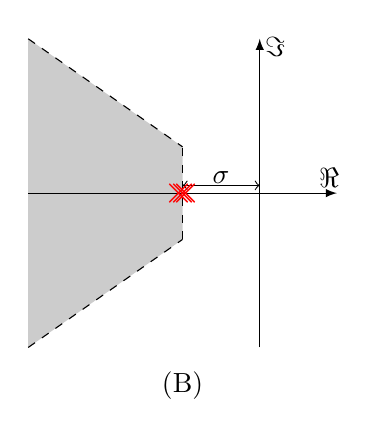
\begin{tikzpicture}[scale=0.98]
				%\draw[help lines,step=1] (0,0) grid (4,4);
				\draw [-latex] (0,2) -- (4,2);
				\draw [-latex] (3,0) -- (3,4);
				\draw [dashed] (0,0) -- (2,1.4);
				\draw [dashed] (0,4) -- (2,2.6);
				\draw [dashed] (2,1.4) -- (2,2.6);
				\draw [<->] (2,2.1) -- (3,2.1);
				\fill [fill opacity=0.2] (0,0) -- (2,1.4) -- (2,2.6) -- (0,4);
					
				\node [align=center] at (3.9, 2.2) {$\Re$};
				\node [align=center] at (3.2, 3.9) {$\Im$};	
				\node [align=center] at (2.5,2.2) {$\sigma$};	
				\node [align=center, red] at (2.05,2) {\Large $\times$};
				\node [align=center, red] at (1.95,2) {\Large $\times$};
				\node [align=center, red] at (2,2) {\Large $\times$};
				
				\node [align=center] at (2,-.5) {(B)};		
			\end{tikzpicture}
			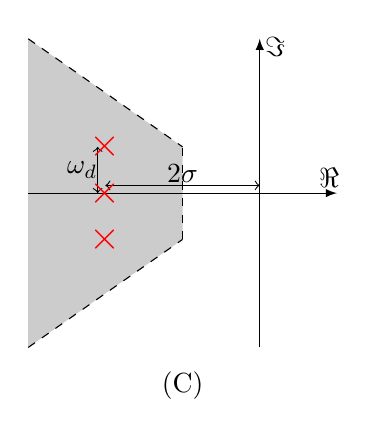
\begin{tikzpicture}[scale=0.98]
				%\draw[help lines,step=1] (0,0) grid (4,4);
				\draw [-latex] (0,2) -- (4,2);
				\draw [-latex] (3,0) -- (3,4);
				\draw [dashed] (0,0) -- (2,1.4);
				\draw [dashed] (0,4) -- (2,2.6);
				\draw [dashed] (2,1.4) -- (2,2.6);
				\draw [<->] (1,2.1) -- (3,2.1);
				\draw [<->] (0.9,2) -- (0.9, 2.6);
				\fill [fill opacity=0.2] (0,0) -- (2,1.4) -- (2,2.6) -- (0,4);
					
				\node [align=center] at (3.9, 2.2) {$\Re$};
				\node [align=center] at (3.2, 3.9) {$\Im$};	
				\node [align=center] at (2,2.25) {$2\sigma$};
				\node [align=center] at (0.7,2.3) {$\omega_d$};	
				\node [align=center, red] at (1,1.4) {\Large $\times$};
				\node [align=center, red] at (1,2.6) {\Large $\times$};
				\node [align=center, red] at (1,2) {\Large $\times$};	
				
				\node [align=center] at (2,-.5) {(C)};	
			\end{tikzpicture}
			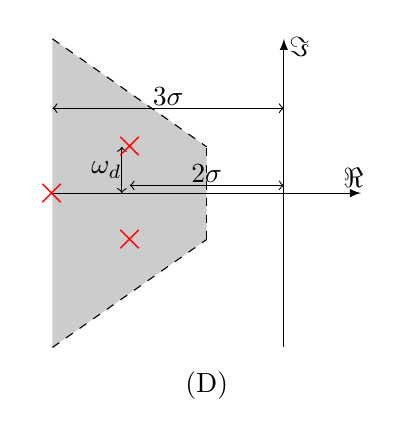
\begin{tikzpicture}[scale=0.98]
				%\draw[help lines,step=1] (0,0) grid (4,4);
				\draw [-latex] (0,2) -- (4,2);
				\draw [-latex] (3,0) -- (3,4);
				\draw [dashed] (0,0) -- (2,1.4);
				\draw [dashed] (0,4) -- (2,2.6);
				\draw [dashed] (2,1.4) -- (2,2.6);
				\draw [<->] (0,3.1) -- (3,3.1);
				\draw [<->] (0.9,2) -- (0.9, 2.6);
				\draw [<->] (1,2.1) -- (3,2.1);
				\fill [fill opacity=0.2] (0,0) -- (2,1.4) -- (2,2.6) -- (0,4);
					
				\node [align=center] at (3.9, 2.2) {$\Re$};
				\node [align=center] at (3.2, 3.9) {$\Im$};	
				\node [align=center] at (1.5,3.25) {$3\sigma$};
				\node [align=center] at (2,2.25) {$2\sigma$};
				\node [align=center] at (0.7,2.3) {$\omega_d$};	
				\node [align=center, red] at (1,1.4) {\Large $\times$};
				\node [align=center, red] at (1,2.6) {\Large $\times$};
				\node [align=center, red] at (0,2) {\Large $\times$};
				
				\node [align=center] at (2,-.5) {(D)};
			\end{tikzpicture}		
			\caption{Quattro diverse configurazioni dei poli in catena chiusa.}
			\label{fig:quattroPoli}				
		\end{figure}		
		
		\begin{wrapfloat}{figure}{R}{0pt}
			\centering		
			\begin{tikzpicture}[scale=0.99, spy using outlines={circle, magnification=4, connect spies}]
					%\draw[help lines,step=.2] (0,0) grid (4,4);
					\begin{axis}[
					grid=major,
			  		xmin=950, xmax=1300, 
			  		ymin=-5, ymax=55,     
			  		xlabel={$t \singleSpacing [s]$},
			  		ylabel={$y \singleSpacing [gradi]$},            
			  		title={Uscite del motore per $d=0$ e $r=50$}, 
			  		xtick={1000,1100,...,1300},
			  		xticklabels={$1$, $1.1$, $1.2$, $1.3$},
			  		ytick={0,10,...,50},
			  		yticklabels={$0$, $10$, $20$, $30$, $40$, $50$},
			  		legend pos=north west,        
			  		legend cell align=left,     
			  		legend entries={(A), (B), (C), (D)},
					]
						\addplot[red] table {./simulazioni/5/poli/out_r_50_A.dat};
						\addplot[green] table {./simulazioni/5/poli/out_r_50_B.dat};
						\addplot[blue] table {./simulazioni/5/poli/out_r_50_C.dat};
						\addplot[orange] table {./simulazioni/5/poli/out_r_50_D.dat};
						
						\coordinate (spypoint) at (115,540);
						\coordinate (magnifyglass) at (126,170);
					\end{axis}
					
				\spy [black, size=3cm] on (spypoint) in node[fill=white] at (magnifyglass);
				\end{tikzpicture}
			\caption{Uscite del motore per le quattro diverse configurazioni dei poli.}
			\label{fig:quattroPoliOuts}					
		\end{wrapfloat}		
			
		\noindent In figura \ref{fig:quattroPoliOuts} sono rappresentate le quattro possibili uscite del sistema per le quattro diverse configurazioni dei poli. Si nota che nessuna delle uscite presenta della sovraelongazione ma per le posizioni dei poli (A) e (B) il tempo di assestamento non rispetta le specifiche. Questo significa che pur essendo teoricamente dentro la zona delle specifiche le approssimazioni fatte non permettono di rispettarle. Poi, nella configurazione (B) il tempo di assestamento minimo non viene rispettato di poco, questo farebbe pensare che il parametro maggiormente approssimato sarebbe $\omega_d$ visto che se tutti i poli si trovano in posizione $-\sigma$ si ottiene appunto quasi l'estremo delle specifiche. Per quanto riguarda (C) e (D) invece le prestazioni sono molto maggiori e sarebbero entrambe configurazioni valide. Si è comunque scelto come migliore la (D) visto che pur avendo una leggerissima sovraelongazione (circa 0,6\%, evidenziata in figura) il tempo di assestamento è leggermente migliore. Scegliendo allora la (D) si eseguono le solite simulazioni per $r=10,50,120$ e $d=\pm0.2$, i risultati  sono riportati in figura \ref{fig:IntegraleDouts}. Come si può notare il sistema si comporta molto bene e le  
		
		\begin{figure}[H]
			\centering
			\includestandalone[width=1\textwidth]{./simulazioni/5_poles_D_only_out} 
			\caption{Uscite del motore con controllore integrale e rumore additivo $d=\pm 0.2$ in configurazione (D).}
			\label{fig:IntegraleDouts}		
		\end{figure}		
		
		\noindent prestazioni sono molto simili per tutte le simulazioni, ovvero tempi di assestamento di poco sotto al decimo  di secondo e sovraelongazioni di circa $0.6 \%$ il valore $r$.
			
			
			
			
			
			
			
			
			
			
			
			
			
			
			
			
			
			
	
	
	
	
	
	
	
	
	
	
	
	\subsection{Verifica sperimentale in laboratorio}
	\label{subsec:LAB}
		
		Si passa alla verifica in laboratorio di quanto fatto fin'ora, in particolare si valuteranno le differenze fra quanto simulato e il dato reale per ciascun sistema di controllo ma soprattutto si  valuterà quale controllore è migliore rispetto agli altri. Per prima cosa si è provveduto a una ritaratura manuale del PID, infatti questo tipo di controllore è piuttosto sensibile agli errori di modello, ma comunque non si è dovuto lavorare molto per la ritaratura, è bastato alzare leggermente il guadagno integrale per rendere il sistema più veloce. Stessa cosa anche per il controllo in feedforward, si è effettuata una prima prova con il valore teorico e misurato l'uscita e per la ritaratura si è semplicemente moltiplicato il valore di $N$ per il rapporto tra $r$ e l'$r$ misurato.
		
		\begin{equation}
			N_{ritarato} = N \cdot \frac{r}{r_{misurato}}
		\end{equation}
		
		\noindent Questo semplice ma efficace sistema ha reso la taratura molto facile e l'errore a regime misurato si è dimostrato essere inferiore all'un per mille. Inoltre si è appurato come si è dovuto modificare il valore di meno di un centesimo rispetto a quello originale, dimostrando che l'errore di modello e/o l'errore sistematico degli strumenti di misura sono bassi. Per quanto riguarda il controllo integrale non si è effettuata nessuna ritaratura della posizione dei poli, ma si è tenuta la configurazione (D). Detto questo si procede allora al confronto dei diversi controllori, le uscite del motore sono riportate in figura \ref{fig:outLAB} mentre in figura \ref{fig:prestazioniLAB} sono riportati due semplici diagrammi che mostrano quale sia effettivamente il miglior controllo. 
		
		
		\begin{figure}[H]
			\centering
			\begin{tikzpicture}[scale=1.07]
				\begin{axis}[
				    xbar,
				    enlarge y limits=0.25,
				    enlarge x limits=0,
				    xmin=0, xmax=11,
				    title={Sovraelongazioni in \%},
				    width=8cm, height=5.9cm,
				    legend style={at={(0.5,-0.15)}, anchor=north,legend columns=-1},
				    %ylabel={\#participants},
				    symbolic y coords={$r=120$,$r=50$,$r=10$},
				    ytick=data,
				    nodes near coords,
				    nodes near coords align={horizontal},
				    reverse legend,
				    ]
					\addplot[green] coordinates {(9.6,$r=120$) (6.8,$r=50$) (9,$r=10$)};
					\addplot[red] coordinates {(0,$r=120$) (0,$r=50$) (1.8,$r=10$)};
					\addplot[blue] coordinates {(0.6,$r=120$) (1.7,$r=50$) (4.8,$r=10$)};
					\legend{integrale \singleSpacing,feedforward \singleSpacing,PID \singleSpacing}
				\end{axis}
			\end{tikzpicture}
			\begin{tikzpicture}[scale=1.07]
				\begin{axis}[
				    xbar,
				    enlarge y limits=0.25,
				    enlarge x limits=0,
				    xmin=0, xmax=0.24,
				    title={Tempi di assestamento in secondi},
				    width=8cm, height=5.9cm,
				    legend style={at={(0.5,-0.15)}, anchor=north,legend columns=-1},
				    %ylabel={\#participants},
				    symbolic y coords={$r=120$,$r=50$,$r=10$},
				    ytick={},
				    yticklabels={},
				    ytick=data,
				    nodes near coords,
				    nodes near coords align={horizontal},
				    reverse legend,
				    ]
					\addplot[green] coordinates{(0.168,$r=120$) (0.171,$r=50$) (0.168,$r=10$)};
					\addplot[red] coordinates {(0.096,$r=120$) (0.092,$r=50$) (0.108,$r=10$)};
					\addplot[blue] coordinates {(0.209,$r=120$) (0.168,$r=50$) (0.176,$r=10$)};
					\legend{integrale \singleSpacing,feedforward \singleSpacing,PID \singleSpacing}
				\end{axis}
			\end{tikzpicture}		
			\caption{Confronto prestazioni mediante l'uso dei tre diversi controllori.}
			\label{fig:prestazioniLAB}	
		\end{figure}
		
		\begin{figure}[H]
			\centering
			\includestandalone[width=1\textwidth]{./simulazioni/LAB_all_out} 
			\caption{Uscite del motore con i tre diversi controllori.}
			\label{fig:outLAB}		
		\end{figure}		
		
		\begin{figure}[H]
			\centering
			\includestandalone[width=1\textwidth]{./simulazioni/LAB_all_in} 
			\caption{Ingressi di controllo con i tre diversi controllori.}
			\label{fig:inLAB}		
		\end{figure}		
		
		\noindent Come si vede il miglior controllo è sempre quello in feedforward ritarato, sia per quanto riguarda il tempo di assestamento sia per quanto riguarda la massima sovraelongazione. Per assurdo è stato anche il controllore più semplice da realizzare, infatti bastano dei semplici comandi \textit{MATLAB} per il posizionamento automatico dei poli e il guadagno di feedforward è stato molto semplice da ritarare. Il controllore PID invece è anch'esso molto semplice ma ha richiesto del tempo per la sua ritaratura, cosa che può diventare anche piuttosto lunga se l'operatore non è abbastanza allenato nel fare questo. Dal controllo integrale invece si ottengono scarse prestazioni, comparabili al PID come tempo di assestamento ma nettamente peggiori come massima sovraelongazione. Ci si aspettava comunque che il controllo integrale fosse lento per la sua natura, infatti una possibile soluzione è quella di utilizzare in accoppiata il feedforward e l'integrale per compensare gli errori di entrambi, ma questo non è stato fatto in questa esperienza. Una ulteriore possibile causa delle scarse prestazioni del controllo integrale, potrebbe essere legata al fatto che la configurazione (D) prevede il posizionamento dei poli molto negativi, incrementando il valore della matrice di retroazione $K$. Infatti, controllando a posteriori il codice MATLAB, si vede come la matrice $K$ abbia valori molto elevati, anche dieci volte superiori a quella del controllo in feedforward. Ciò ha portato molto probabilmente a una amplificazione dei rumori di misura e quindi un non corretto funzionamento del sistema di controllo. Una curiosità che si nota in figura \ref{fig:outLAB} è che prima che il riferimento cambi di stato da $0$ a $r$ è che l'uscita rimane poco sopra allo zero, questo è un effetto dell'attrito di stacco, completamente trascurato in fase di modellizzazione. Altra cosa è che gli ingressi del PID sono molto più stabili rispetto a quanto ottenuto in simulazione, pur rimanendo comunque più oscillanti rispetto al feedforward e l'integrale. \newline
		
		\noindent In conclusione questa esperienza di laboratorio fornisce diversi spunti di riflessione. Innanzitutto, fin da subito è stato evidente come un controllore progettato per rispettare le specifiche in simulazione non necessariamente farà altrettanto una volta provato sul processo reale. Ciò può essere dovuto ad eccessive semplificazioni nella fase di modelizzazione del processo, a dati nominali non fedeli alla realtà o semplicemente a disturbi impossibili da eliminare nei processi veri. Ciò però non significa che la progettazione su modello di un controllore sia completamente inutile. Infatti si è notato come nella maggior parte dei casi l’andamento di ingressi e uscite previste avesse un andamento molto simile a quello effettivamente misurato in laboratorio. Tuttavia una fase di ritaratura dei parametri si è resa necessaria per riuscire a rispettare le specifiche imposte e ciò accade spesso nella pratica. In sostanza, quindi, la fase di modellizzazione è necessaria per poter capire quale sarà approssimativamente il comportamento del nostro sistema in catena chiusa e decidere quale sia il miglior controllo da attuare. Ma è anche vero che non ha solitamente senso effettuare una troppo scrupolosa taratura dei parametri di controllo sul modello perché spesso il sistema fisico si comporterà diversamente da quanto previsto.   
		
		
		
		
		